\section{Forward Kinematics using the Denavit-Hartenberg scheme}
Forward kinematics allow us to express the pose of a mechanism given its actuator parameters such as the angle of a joint or the number of rotations of its wheel as well as their derivatives including speed and accleration, without taking into account the forces that cause the motion. So far, we have considered the forward kinematics of wheeled mechanisms and simple arms. Whereas we could derive kinematic equations of simple mechanisms using basic trigonometry, we can also think about the forward kinematics as a chain of homogenous transformations that express mobile coordinate systems in a static one usually mounted at the base of a manipulator or a fixed position in the room. Deriving these transformations can be confusing and can be facilitated by following a ``recipe'' such as conceived by Denavit and Hartenberg. The so-called Denavit-Hartenberg (DH) \index{Denavit-Hartenberg parameters}scheme has evolved as quasi-standard and can easily be automatized, i.e., applied to a 3D model of a robotic arm, e.g. 

A manipulating arm consists of links that are connected by joints. Joints can be either rotational or prismatic, i.e., change their length and thus providing additional degrees of freedom. Knowing the length of all rigid links, the position of the manipulators end-effector is fully described by its joint angles and joint offset (for prismatic joints).

%In industrial manipulators, the number of joints is usually equal to the degrees of freedom of the manipulator. As most manipulators are holonomic, the forward kinematics allow you---unlike on non-holonomic wheeled platforms---to directly relate absolute positions of joints with absolute positions in Cartesian space. It is also possible to derive equations that relate the speed of the joints to speed in Cartesian space. Like for wheeled platforms, this can be achieved via a Jacobian matrix.  At certain positions, the mapping provided by the Jacobian is not invertible, i.e., some velocities in Cartesian space are unachievable. These points are called singularities.

\screencast{http://youtu.be/rA9tm0gTln8}{denavithartenberg}
In oder to use the DH-convention, we first need to define a coordinate system at each joint. We chose the z-axis to be the axis of rotation for a hinge joint and the axis of translation for a prismatic joint. We can now find the common normal between the z-axes of two subsequent joints, i.e., a line that is orthogonal to each z-axis and intersects both. With the direction of the x-axis at the base arbitrary, subsequent x-axis are chosen such that they lie on the common normal shared between two joints. Whereas the direction of the z-axis is given by the positive direction of rotation (right hand rule), the x-axis points away from the previous joint. This allows defining the y-axis using the right-hand rule. Note that these rules, in particular the requirement that $x$-axes lie along the commom normal, might result in coordinate systems with their origins outside the joint. %Rather, the origin of joint $n$ is at the intersection of   

The transformation between two joints is then fully described by the following four parameters:
\begin{enumerate}
\item the length $ r$ of the common normal between the $z$-axes of two joints $i$ and $i-1$ (link length)
\item The angle $ \alpha$ between the z-axes of the two joints with respect to the common normal (link twist), i.e., the angle between the old and the new $z$-axis, measured about the common normal.
\item The distance $d$ between the joint axes (link offset), i.e., the offset along the previous $z$-axis to the common normal.
\item The rotation $ \theta$ around the common axis along which the link offset is measured (joint angle), i.e., the angle from the old $x$-axis to the new $x$-axis, about the previous $z$-axis.
\end{enumerate}

Two of the D-H parameters describe the link between the joints, and the other two describe the link's connection to a neighboring link. Depending on the link/joint type, these numbers are fixed or can be controlled. For example, in a revolute joint $ \theta$ is the varying joint angle, while all other quantities are fixed.  Similarly, for a prismatic joint $ d$ is the joint variable. An example of two revolute joints is shown in Figure \ref{fig:denavit}.

\begin{figure}
	\centering
		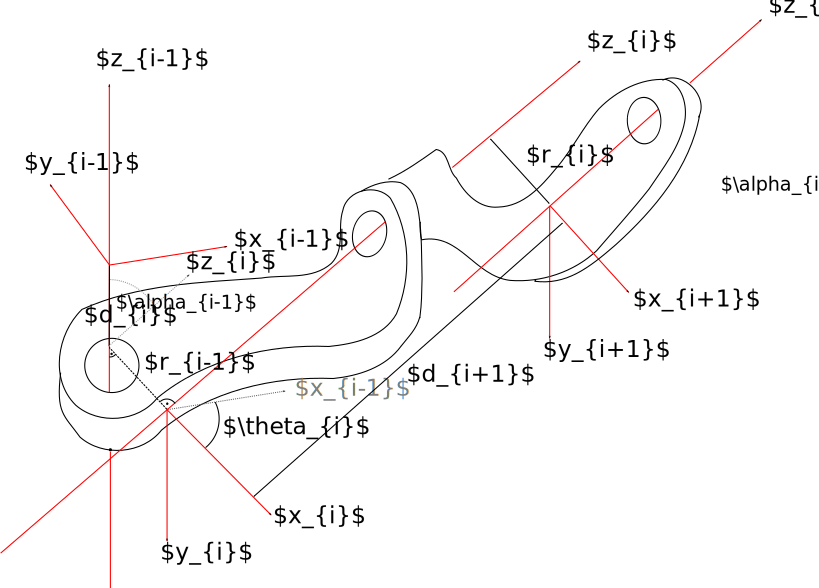
\includegraphics[width=\textwidth]{figs/denavit-hartenberg}
	\caption{Example of selected Denavit-Hartenberg parameters for three revolute joints. The z-axes of joint $i$ and $i+1$ are parallel.
	\label{fig:denavit}}
\end{figure}



The coordinate transform from one link ($ i-1$) to another ($i$) can now be constructed  using the following matrix:
\begin{eqnarray}{ll}
\nonumber
_{n-1}^nT=&
\left(
\begin{array}{ccc|c}
\cos \theta_n & -\sin \theta_n \cos\alpha_n & \sin\theta_n \sin\alpha_n & r_n \cos\theta_n\\
\sin \theta_n & \cos\theta_n \cos\alpha_n & -\cos\theta_n\sin\alpha_n & r_n \sin\theta_n\\
0 & \sin\alpha_n & \cos\alpha_n & d_n\\
\hline
0 & 0 & 0 & 1
\end{array}
\right)\\
&=
\left(
\begin{array}{c|c}
R & t\\
\hline
0 \quad 0 \quad 0 & 1
\end{array}
\right)
\end{eqnarray}
with the rotation matrix $R$ and the translation vector $t$. This matrix can be constructed by a series of rotations and translations, one for each DH parameter:
\begin{equation}
_{n-1}^nT=T_z'(d_n)\dot R_z'(\theta_n) \dot T_x(r_n) \dot R_x(\alpha_n)
\end{equation}
with
\begin{equation}
T_z'(d_n)=
\left(
\begin{array}{ccc|c}
1 & 0 & 0 & 0\\
0 & 1 & 0 & 0\\
0 & 0 & 1 & d_n\\
\hline
0 & 0 & 0 & 1
\end{array}
\right)
\enskip
R_z'(\theta_n)=\left(
\begin{array}{ccc|c}
\cos\theta_n & -\sin\theta_n & 0 & 0\\
\sin\theta_n & \cos\theta_n & 0 & 0\\
0 & 0 & 1 & 0\\
\hline
0 & 0 & 0 & 1
\end{array}
\right)
\end{equation}
and
\begin{equation}
T_x(r_n)=
\left(
\begin{array}{ccc|c}
1 & 0 & 0 & r_n\\
0 & 1 & 0 & 0\\
0 & 0 & 1 & 0\\
\hline
0 & 0 & 0 & 1
\end{array}
\right)
\enskip
R_x(\alpha_n)=\left(
\begin{array}{ccc|c}
1 & 0 & 0 & 0\\
0 & \cos\alpha_n & -\sin\alpha_n & 0\\
0 & \sin\alpha_n & \cos\alpha_n & 0\\
\hline
0 & 0 & 0 & 1
\end{array}
\right)
\end{equation} 
These are a translation of $d_n$ along the previous z-axis ($T_z'(d_n)$), a rotation of $\theta_n$ about the previous z-axis ($R_z'(\theta_n)$), a translation of $r_n$ along the new $x$-axis ($T_x(r_n)$)and a rotation of $\alpha_n$ around the new $x$-axis ($R_x(\alpha_n)$).

Like for any homogeneous transfrom, the inverse $_{n-1}^nT^{-1}n$ is given by
\begin{equation}
^{n-1}_nT=\left(
\begin{array}{c|c}
R^{-1} & -R^{-1}T\\
\hline
0 \quad 0 \quad 0 \quad 1
\end{array}
\right)
\end{equation}
with the inverse of $R$ simply being its transpose.

\section{Inverse Kinematics of Complex Mechanisms}\label{sec:advinvkinematics}
The forward kinematics of a system are given by a transformation matrix from the base of a manipulator (or a corner of the room) to the end-effector of a manipulator (or a mobile robot). As such, they are an exact description of the pose of the robot. In order to find the joint angles that lead to the desired pose, we will need to solve these equations for joint angles as a function of the desired pose. This is possible for simple kinematics, but gets quickly out of hand for complex kinematics; it is not possible for non-holonomic mobile robots, which require us to find a sequence of actuation commands. This section provides a solution for both these problems.

\subsection{Solvability}
As the resulting equations are heavily non-linear, it makes sense to briefly think about whether we can solve them at all for specific parameters before trying. Here, the workspace of a robot becomes important. The workspace is the sub-space that can be reached by the robot in any orientation. Clearly, there will be no solutions for the inverse kinematic problem outside of the workspace of the robot.

A second question to ask is how many solutions we actually expect and what it means to have multiple solutions geometrically. Multiple solutions to achieve a desired pose correspond to multiple ways in which a robot can reach a target. For example a three-link arm that wants to reach a point that can be reached without fully extending all links (leading to a single solution), can do this by  folding its links in a concave and a convex fashion. How many solutions there are for a given mechanism and pose quickly becomes non-intuitive. For example a 6-DOF arm can reach certain points with up to 16 different conformations.

\subsection{Numerical Techniques: Inverse Jacobian}\label{sec:invjac}
The above example (Figure \ref{fig:fwk2dofarm}) involved only two free parameters, but was already pretty complex to solve analytically if the end-effector pose was not specified. One can imagine that things become very hard with more degrees of freedom or more complex geometries. (Mechanisms in which some axes intersect are simpler to solve than others, for example.) Fortunately, there are simple numerical techniques that work reasonably well. One of them known is as \emph{Inverse Jacobian}\index{Inverse Jacobian} technique:

As we can easily calculate the resulting pose for every possible joint angle combination using the forward kinematic equations, we can calculate the error between desired and actual pose. This error actually provides us with a direction that the end-effector needs to move. As we only need to move tiny bits at a time and can then re-calculate the error, this is an attractive method to generate a trajectory that moves the arm to where we want it go and thereby solving the inverse kinematics problem.

In order to do this, we need an expression that relates the desired speed of the robot's end-effector, i.e., the direction in which we want to move, to the speed at which we need to change our joints. Let the translational speed of a robot be given by 
\begin{equation}
v=\left(\begin{array}{c}
\dot{x}\\
\dot{y}\\
\dot{z}
\end{array}
\right).
\end{equation}

 As the robot can potentially not only translate, but also rotate, we also need to specify its angular velocity. Let these velocities be given as a vector 
\begin{equation}
\omega=\left(\begin{array}{c}
\omega_x\\
\omega_y\\
\omega_z
\end{array}
\right).
\end{equation}

This notation is also called a \emph{velocity screw}.\index{Screw (velocity)}\index{Velocity Screw} %By convention, the speed of rotation is given by the magnitude (or length) of this vector. 
We can now write translational and rotational velocities in a 6x1 vector as $ (v \quad \omega)^T$. Let the joint angles/positions be $j=(j_1, \ldots, j_n)$.

Given a relationship between end-effector velocities $\dot{j}$ and joint velocities $J$, we can write
\begin{equation}
 (v \quad \omega)^T=J(\dot{j}_1,\ldots,\dot{j}_n)^T
\end{equation}

with $ n$ the number of joints. $J$ is also known as the Jacobian matrix \index{Jacobian Matrix} and contains all partial derivatives that relate every joint angles to every velocities. In practice, $J$ looks like

\begin{equation}
\left(\begin{array}{c}v\\\omega\end{array}\right)=\left(\begin{array}{ccc}\frac{\partial{x}}{\partial{j_1}} & \ldots & \frac{\partial{x}}{\partial{j_n}}\\\vdots & \quad & \vdots\\\frac{\partial{\omega_z}}{\partial{j_1}} & \ldots & \frac{\partial{\omega_z}}{\partial{j_n}}\end{array}\right)(j_1,\ldots,j_n)^T
\end{equation}

This notation is important as it tells us how small changes in the joint space will affect the end-effector's position in cartesian space. Better yet, the forward kinematics of a mechanism can always be calculated, as well as their analytical derivatives, allowing us to calculate numerical values for the entries of matrix $J$ for every possible joint angle/position.

It would now be desirable to just invert $J$ in order to calculate the necessary joint speeds for every desired end-effector speeds. Unfortunately, $ J$ is only invertible if there are exactly 6 independent joints, so that $ J$ is quadratic and has full rank. If this is not the case, we can use the pseudo-inverse instead:
\begin{equation}
J^+=\frac{J^T}{JJ^T}=J^T(JJ^T)^{-1}
\end{equation}
As you can see, $J^T$ cancels from the equation leaving $1/J$, while being applicable to non-quadratic matrices.

This solution might or might not be numerically stable, depending on the current joint values. If the inverse of $J$ is mathematically not feasible, we speak of a \emph{singularity}\index{Singularity} of the mechanism. This happens for example when two joint axes line up, therefore effectively removing a degree of freedom from the mechanism, or at the boundary of the workspace. Mathematically speaking the rank of the Jacobian is smaller than six.

We can now write a simple feedback controller that drives our error $e$ as the difference between desired and actual position to zero:
\begin{equation}
\Delta{j}=-J^+e
\end{equation}
That is, we move each joint a tiny bit into the direction that minimizes $e$.
It can be easily seen that the joint speeds are only zero if $e$ has become zero. A problem arises, however, when the end-effector has to go through a singularity to get to its goal. Then, the solution to $ J^+$ ``explodes'' and joint speeds go to infinity. In order to work around this, we can introduce damping to the controller.

This can be achieved by not only minimizing the error, but also the joint velocities. Thus, the minimization problem becomes
\begin{equation}
\|J\Delta j-e\|+\lambda^2\|\Delta j\|^2
\end{equation}

where $\lambda$ is some constant. One can show that the resulting controller that achieves this has the form
\begin{equation}
\Delta j=(J^TJ+\lambda^2 I)^{-1}J^+e
\end{equation}

This is known as the \emph{Damped Least-Squares} method.\index{Damped Least-Squares Method} Problems with this approach are local minima and singularities of the mechanism, that might render this solution infeasible.

Using a feedback controller to solve the inverse kinematic problem for a mobile robot is actually even simpler. Ignoring the problem of converting a translational and rotational velocity of the form $(\dot{x} \dot{theta})^T$ into actual wheel-speeds, we can calculate the error $\rho$ in distance and $\alpha$ in bearing to a desired pose. We can now calculate speeds that are proportional to these errors by
\begin{eqnarray}
\dot{x} &= p_1 \rho\\
\dot{\theta} &= p_2 \alpha
\end{eqnarray}
which will let the robot drive in a curve until it reaches the desired position. 




\section*{Take-home lessons}

\begin{itemize}
\item Forward kinematics are equivalent to finding a coordinate transform from a world coordinate system into a coordinate system on the robot. Such a transform is a combination of a (3x1) translation vector and a (3x3) rotation matrix that consists of the unit vectors of the robot coordinate system. Both translation and rotation can be combined into a 4x4 homogeneous transform matrix.
\item Forward and Inverse Kinematics of a mobile robot are performed with respect to the speed of the robot and not its position.
\item For calculating the effect of each wheel on the speed of the robot, you need to consider the contribution of each wheel independently.
\item Calculating the inverse kinematics analytically becomes quickly infeasible. You can then plan in configuration space of the robot using path-planning techniques.
\item The inverse kinematics of a robot involves solving the equations for the forward kinematics for the joint angles. This process is often cumbersome if not impossible for complicated mechanisms.
\item A simple numerical solution is provided by taking all partial derivatives of the forward kinematics in order to get an easily invertible expression that relates joint speeds to end-effector speeds.
The inverse kinematics problem can then be formulated as feedback control problem, which will move the end-effector towards its desired pose using small steps. Problems with this approach are local minima and singularities of the mechanism, that might render this solution infeasible.
\end{itemize}

\section*{Exercises}\small
\subsection*{Coordinate systems}
\begin{enumerate}
\item 
\begin{enumerate}
 \item Write out the entries of a rotation matrix $^A_BR$ assuming basis vectors $X_A$, $Y_A$, $Z_A$, and $X_B$, $Y_B$, $Z_B$. 
 \item Write out the entries of rotation matrix $^B_AR$.
 \end{enumerate} 
\item Assume two coordinate systems that are co-located in the same origin, but rotated around the z-axis by the angle $\alpha$. Derive the rotation matrix from one coordinate system into the other and verify that each entry of this matrix is indeed the scalar product of each basis vector of one coordinate system with every other basis vector in the second coordinate system.  
\item Consider two coordinate systems $\{B\}$ and $\{C\}$, whose orientation is given by the rotation matrix $^C_BR$ and have distance $^BP$. Provide the homogenous transform $^C_BT$ and its inverse $^B_CT$. 
\item Consider the frame $\{B\}$ that is defined with respect to frame $\{A\}$ as $\{B\}=\{^A_BR, ^AP\}$. Provide a homogeneous transfrom from $\{A\}$ to $\{B\}$.
\end{enumerate}

\subsection*{Forward and inverse kinematics}
\begin{enumerate}
\item Consider a differential wheel robot with a broken motor, i.e., one of the wheels cannot be actuated anymore. Derive the forward kinematics of this platform. Assume the right motor is broken.
\item The forward kinematics of a differential-wheel platform are given by 
\begin{equation}
\nonumber
\left(\begin{array}{c}
\dot{x}_r\\
\dot{y}_r\\
\dot{\theta}
\end{array}\right)
=
\left(\begin{array}{c}
\frac{r\dot{\phi}_l}{2}+\frac{r\dot{\phi_r}}{2}\\
0\\
\frac{r\dot{\phi}_r}{d}-\frac{r\dot{\phi_l}}{d}
\end{array}\right)
\end{equation}
Derive an expression for $\dot{\phi}_l$ and $\dot{\phi}_r$ as a function of the desired speeds $\dot{x}_r$ and $\dot{y}_r$. 
\item Consider a tri-cycle with two independent standard wheels in the rear and the stearable, driven front-wheel. Chose a suitable coordinate system and use $\phi$ as the steering wheel angle and wheel-speed $\dot{\omega}$. Provide forward and inverse kinematics. 
\end{enumerate}
\normalsize